\section{Durchführung}
\label{sec:Durchführung}

% Was wurde gemessen bzw. welche Größen wurden variiert?

Alle folgenden Messungen werden mit einem Röntgengerät, wie dem in \autoref{fig:geraet} durchgeführt.

\begin{figure}
    \centering
    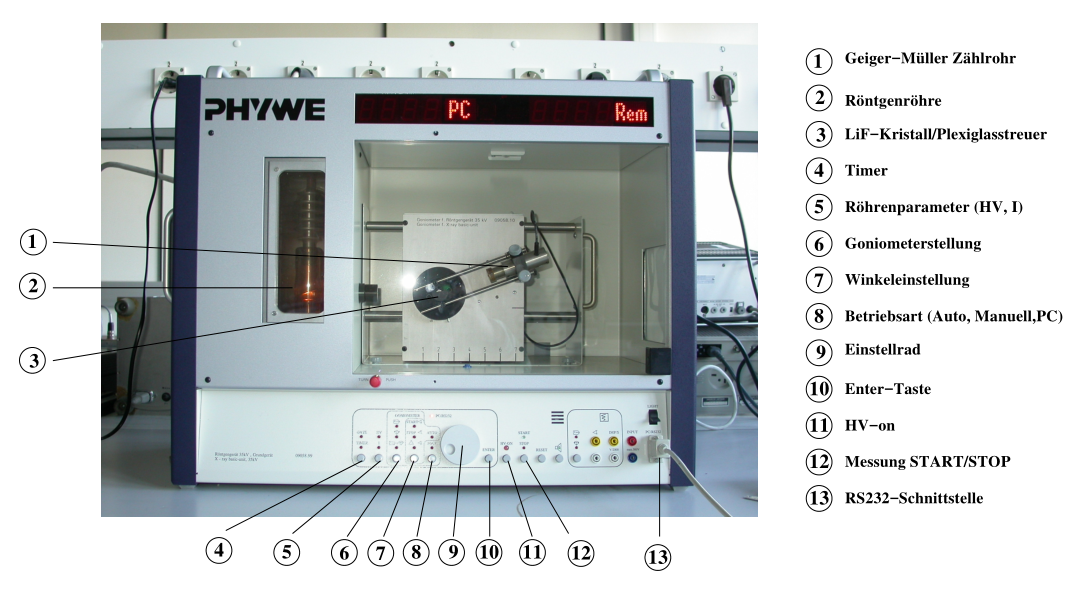
\includegraphics[width=\textwidth]{images/bild4.png}
    \caption{Röntgengerät mit Cu-Röntgenröhre, LiF-Kristall und Geiger-Müller Zählrohr}
    \label{fig:geraet}
\end{figure}

Die meisten Abläufe laufen automatisch ab, sodass nur die richtigen Einstellungen getätigt werden müssen.
Als Messgerät wird das Röntgengerät eingestellt.
Drehwinkel, Kristallwinkel und Integrationszeit müssen alle einstellbar sein.
Vor dem Experiment wird die Beschleunigungsspannung $U_\text{B}$ auf $\SI{35}{\kilo\volt}$ gestellt.
Der Emissionsstrom $I$ soll $\SI{1}{\milli\ampere}$ betragen.
Beide Werte werden im Laufe des Versuches nicht mehr verändert.
LiF-Kristall und die $\SI{1}{\milli\meter}$ Blende müssen beide montiert werden.
Für die Schlitzblende vor dem Geiger-Müller Zählrohr ist es wichtig, dass sie senkrecht zur Drehrichtung eingestellt ist, da sonst zu viele Röntgenstrahlen auf einmal gezählt werden würden, was das Ergebnis verfälschen würde.

\subsection{Überprüfung der Bragg-Bedingung}
\label{ssec:bragg}

Zunächst wird die Bragg-Bedingung überprüft, dafür wird der Kristallwinkel $\theta$ auf $\SI{14}{\degree}$ gestellt.
Das Geiger-Müller Zählrohr soll dann von $\SI{26}{\degree}$ bis $\SI{30}{\degree}$ in $\SI{0.1}{\degree}$ Schritten messen. 
Die Integrationszeit beträgt dabei immer $\SI{5}{\second}$.
Es werden alle Winkel mit ihren Intensitäten notiert.

\subsection{Analyse des Emissionsspektrums einer Cu-Röntgenröhre}
\label{ssec:kupfer}

Für die Messung des Emissionsspektrums wird $\theta$ auf $\SI{8}{\degree}$ gesetzt und von dort bis zu $\SI{25}{\degree}$ vergrößert.
Dies geschieht in $\SI{0.1}{\degree}$-Schritten, wobei die Integrationszeit $\SI{10}{\second}$ beträgt.
Auch hier werden alle Werte mit ihren entsprechenden Intensitäten notiert.

\subsection{Analyse der Absorptionsspektren}
\label{ssec:spektrum}

Zuletzt werden Absorber vor das Geiger-Müller Zählrohr gesetzt.
Es werden ingesesamt Absorptionsspektren aus sechs verschiedenen Elementen verwendet.
Alle Elemente werden in anderen Winkelbereichen gemessen:
Brom von $\SI{12.8}{\degree}$ bis $\SI{14.3}{\degree}$, Gallium von $\SI{17.0}{\degree}$ bis $\SI{19.0}{\degree}$, Rubidium von $\SI{11.2}{\degree}$ bis $\SI{12.5}{\degree}$, Strontium von $\SI{10.5}{\degree}$ bis $\SI{12.0}{\degree}$, Zink von $\SI{18.0}{\degree}$ bis $\SI{19.5}{\degree}$ und Zirkonium von $\SI{9.5}{\degree}$ bis $\SI{11.0}{\degree}$.
Bei allen Elementen werden die Winkel nach $\SI{20}{\second}$ um $\SI{0.1}{\degree}$ vergrößert.
Es werden für alle verschiedenen Absorber die Intensitäten zu den Winkeln notiert.